\chapter{Preliminary Work}
\label{chap:prelim_work}
As preliminary work, several steps were taken to evaluate the validity of the proposed research.
To aid in this task a metric was be developed for the evaluation of the nonlinear convergence of a time-step size insensitive solution.
In order to determine the effects of nonlinear convergence upon the time-step size insensitivity of a solution, the \cobra{} software was modified to enable an iterative global Newton's method.
To aid in the development of the nonlinear convergence metric and the nonlinear solver, a novel operator-based scaling has been developed to obtain meaningful convergence thresholds.
The scaling of the nonlinear residual is typically done in an arbitrary fashion; a scaling factor that is intrinsically linked to the physics of interest was developed.
This scaling produces a non-dimensionalized residual whose magnitude is relative to the physical sources and sinks on a per equation basis. 
Two test problems were developed to show that the nonlinear convergence metric can identify situations where a time-step size insensitive simulation may not satisfy the discrete nonlinear equations.
%--------------------------------------------------------------------------------------------------------------------------------------------------------------------
%--------------------------------------------------------------------------------------------------------------------------------------------------------------------
%--------------------------------------------------------------------------------------------------------------------------------------------------------------------
%--------------------------------------------------------------------------------------------------------------------------------------------------------------------
%--------------------------------------------------------------------------------------------------------------------------------------------------------------------
%--------------------------------------------------------------------------------------------------------------------------------------------------------------------
%--------------------------------------------------------------------------------------------------------------------------------------------------------------------
\section{Nonlinear \cobra{} Implementation}
\label{sect:nl_cobra}
The first stage of preliminary work was to modify the \cobra{} software.
As obtained, the \cobra{} software was a single-shot linearization version of the semi-implicit method.
In order to evaluate the subdomain nonlinear refinement algorithm, \cobra{} needed to be converted to include a fully iterative Newton solver based upon a linesearch globalization strategy.
When it is necessary to distinguish between the single-shot linearization algorithmic implementation of \cobra{} and the iterative nonlinear \cobra{} implementation, the former shall be referred to as legacy mode and the latter as nonlinear mode.
As such, the objectives of this work were to modify the software to be able do the following:

\begin{itemize}
\item{Create a data framework for constructing vector quantities such as $\vec{x}^{k}$ and $\vec{F}$.}
\item{Correctly evaluate $\vec{F}(\vec{x}^{k})$ and $\vec{J}(x^{k})$.}
\item{Implement a globalization strategy for Newton's method.}
\end{itemize}

\cobra{} utilized a single-shot linearization Newton method for its solution technique.
As a result of that design decision, certain memory saving techniques were employed in the construction of the software that precluded the idea of more than one Newton step.
In particular, there was the implicit assumption within the software that the current Newton iterate, $\vec{x}^{n+1, 0}$, was the old-time variable $\vec{x}^{n}$.
This design decision required the vetting of all subroutines involved with the evaluation of the components of both the nonlinear residual and the Jacobian.
In addition, the assumption that $\vec{x}^{n+1, k} = \vec{x}^{n}$ produced source code that was inconsistent with an iterative Newton method.
This required that the source code be modified to reflect the intended discretization of the governing conservation laws.
To do this, areas had to be identified where: there were implicit cancellation of terms, the new-time variables were used in place of old-time variables, and the old-time variables were used in place of new-time variables.
Where appropriate, the software was changed to reflect the distinction between old-time and iterate variables and to introduce terms that had been assumed to be equal to zero.

Once the appropriate variables were used for the evaluation of the nonlinear residuals and the Jacobian, a Newton loop was introduced to allow multiple Newton steps.
\alg{alg:nl_cobra} contains the current algorithmic implementation of the nonlinear semi-implicit method.

\begin{algo}[H]
\caption{Nonlinear \cobra{} solution algorithm.}
\label{alg:nl_cobra}
\setlength{\baselineskip}{0.625\baselineskip}
\begin{algorithmic}[1]
\Require $\vec{x}^{0}$ and $t^{0}$
\Set $n = 0$
\Loop \; Transient Loop
    \State $t^{n+1} : = t^{n} + \Delta t$
    \State $k = 0$
    \Define $\vec{x}^{n+1,0}$
	\Calculate $\vec{F}(\vec{x}^{n+1,0})$ and $\vec{J}(\vec{x}^{n+1,0})$
    \Loop \; Newton Loop
		\Calculate $\vec{\delta x} = - \vec{J}^{-1}\cdot\vec{F}$
		$j = 0$		
		\Calculate $\vec{x}^{n+1,k+1,j}$
		\Calculate $\vec{F}(\vec{x}^{n+1,k+1,j})$
		\Loop \; Globalization Loop
			\If{ Globalization loop termination criteria not met}
				\Calculate $\lambda_j$
				\Calculate $\vec{x}^{n+1,k+1,j+1} = \vec{x}^{n+1,k} + \lambda \vec{\delta x}$
				\Calculate $\vec{F}(\vec{x}^{n+1,k+1,j+1})$
				\State $j = j + 1$			
			\Else
				\Calculate $\vec{J}(\vec{x}^{n+1,k+1,j})$
				\Exit Globalization Loop
			\EndIf
		\EndLoop			
		\If{ Newton loop termination criteria met}
			\Exit Newton Loop
		\EndIf
	\EndLoop
	\State $n = n + 1$
\EndLoop
\end{algorithmic}
\end{algo}

In \alg{alg:nl_cobra}, there are three steps that require discussion.
First is the Newton Loop termination criteria.
There are three Newton loop termination mechanisms, listed below.

\begin{enumerate}
\item{$k > k_{\,\text{MAX}}$}
\item{$||(\vec{S}^{k+1})^{-1}\vec{F}^{k+1}||_{\infty} \leq F_{\text{ABS}}$}
\item{$||(\vec{D}^{k+1})^{-1}\vec{\delta x}^{k}||_{\infty} \leq \delta_{\text{ABS}}$}
\end{enumerate}

Current values for $k_{\,\text{MAX}}$, $F_{\text{ABS}}$ and $\delta_{\text{ABS}}$ are $35$, $1.0$E$-05$, and $1.0$E$-10$, respectively.
The scaling vectors, $\vec{S}$ and $\vec{D}$, will be addressed later.

The globalization strategy implemented in \cobra{} is a linesearch algorithm \cite{Dennis1996}.
The two globalization loop termination criteria are:

\begin{enumerate}
\item{$\frac{1}{2}||\vec{F}^{k+1, j}||^{2}_{2} < \frac{1}{2}||\vec{F}^{k}||^{2}_{2} - \alpha ||\vec{F}^{k}||^{2}_{2}$ }
\item{$||\lambda_{j+1} \vec{\delta x}^{k}||_{\infty} < \delta_{\text{abs}}$}
\end{enumerate}

If neither of the loop termination criteria are met, then the step-length parameter, $\lambda_j$ is calculated.
On the first pass through the globalization loop within a given Newton step, a quadratic backtracking model is adopted.
On subsequent passes, a cubic-backtracking model is used.
 
Since vector forms of the nonlinear residual and the independent parameters are used in determining nonlinear convergence and in the globalization algorithm, they needed to be easily manipulated.
A subroutine was written to gather the discrete variables of the independent parameters into a single vector.
Additional source code modifications were necessary to construct and gather the components of the nonlinear residual.

%--------------------------------------------------------------------------------------------------------------------------------------------------------------------
%--------------------------------------------------------------------------------------------------------------------------------------------------------------------
%--------------------------------------------------------------------------------------------------------------------------------------------------------------------
%--------------------------------------------------------------------------------------------------------------------------------------------------------------------
%--------------------------------------------------------------------------------------------------------------------------------------------------------------------
%--------------------------------------------------------------------------------------------------------------------------------------------------------------------
%--------------------------------------------------------------------------------------------------------------------------------------------------------------------
\section{Operator-Based Scaling}
\label{sect:operator_scaling}
In order to determine the degree to which a state vector, $\vec{x}$, satisfies \eqref{eqn:conservation_equations}, the use of the nonlinear residual is required.
However, due to the units of the residuals for the different conservation equations, their magnitudes can vary by orders of magnitude. 
For a given continuity volume, the nonlinear residual will have six components: four for the conservation of mass and two for the conservation of energy.
For each momentum volume, the three conservation of momentum equations will form the three components of the nonlinear residual.
These residuals have the units of the conserved quantities for their corresponding PDEs; \tab{tab:scaling_units_scales} shows the units for the different conservation equations.

\begin{table}[ht]
\centering
\begin{tabular}{@{}l c r @{}} \toprule
Residual & Units \\
\midrule
Conservation of the \NCG{} Field Mass                  & [ lb$_m$ ] \\
Conservation of the Continuous Liquid Water Field Mass & [ lb$_m$ ] \\
Conservation of the Entrained Liquid Water Field Mass  & [ lb$_m$ ] \\
Conservation of the Water Vapor Field Mass             & [ lb$_m$ ] \\
Conservation of the Gaseous Phase Enthalpy             & [ BTU ]    \\
Conservation of the Liquid Phase Enthalpy              & [ BTU ]    \\
Conservation of the Continuous Liquid Field Momentum   & [ $\frac{\text{lb}_{\text{m}} \text{ft}}{\text{s}}$ ] \\
Conservation of the Entrained Liquid Field Momentum & [ $\frac{\text{lb}_{\text{m}} \text{ft}}{\text{s}}$ ] \\
Conservation of the Gaseous Phase Momentum & [ $\frac{\text{lb}_{\text{m}} \text{ft}}{\text{s}}$ ] \\
\bottomrule  
\end{tabular}
\caption{Residuals and their units.}
\label{tab:scaling_units_scales}
\end{table}

Due to the range of magnitudes of these residuals, it is important to choose a proper scaling factor.
A challenge that has been addressed in this work is the development of a method for scaling of these residuals that is based upon the physics of interest during a time-step.
In constructing this scaling factor, it was determined that following characteristics were desirable:
\begin{itemize}
\item{$(S_{i}^{k})^{-1} F^{k}_i \approx 1$ when $\vec{x}^{k}$ is a "poor" solution.}
\item{$(S_{i}^{k})^{-1} F^{k}_i \rightarrow 0$ when phase $i$ disappears.}
\item{$0 \leq (S_{i}^{k})^{-1} F^{k}_{i} \leq 1 $ for all values of $\vec{x}^{k}_i$.}
\end{itemize}

The scaling used in this work is an operator based approach.
The governing PDEs can be viewed as a collection of operators, both linear and nonlinear, acting upon the vector of independent parameters.
The summation of these operators must balance to zero for the nonlinear equation to be satisfied.

To illustrate the scaling procedure, we shall consider \eqref{eqn:conservation_of_liq} for a simply connected continuity cell without inter-field mass transfer.
Assume that the entire channel single-phase and in thermodynamics equilibrium such that the macroscopic densities on either side of this single cell are the same.

\begin{equation}
F = \left(\alpha_k \rho_k\right)^{n+1} - \left( \alpha_k \rho_k \right)^n - \frac{\Delta t}{V} \left( \frac{<\alpha^{n}_k \rho^{n}_k>^{n}_{d} }{<\alpha_k \rho_k>^{n}_{a}} V^{n+1}_{j-1} \right)
\end{equation}

In this equation there are three physically meaningful quantities: the temporal difference, the mass flowing into the cell, and mass flowing out of the volume. 

%--------------------------------------------------------------------------------------------------------------------------------------------------------------------
%--------------------------------------------------------------------------------------------------------------------------------------------------------------------
%--------------------------------------------------------------------------------------------------------------------------------------------------------------------
%--------------------------------------------------------------------------------------------------------------------------------------------------------------------
%--------------------------------------------------------------------------------------------------------------------------------------------------------------------
%--------------------------------------------------------------------------------------------------------------------------------------------------------------------
%--------------------------------------------------------------------------------------------------------------------------------------------------------------------
\section{Temporal Convergence}
\label{sect:temporal_convergence}

An important factor in thermal-hydraulic safety analysis is the temporal convergence of the solution.
First, a definition of a temporally converged solution is required.
In theory, a temporally converged solution is one where the local truncation error due to the discrete approximation of the temporal integral is orders of magnitude below both the engineering scales of interest and precision of the physical models being used in the simulation.
Unfortunately, the precise measurement of the error in a simulation requires that an analytic solution be available for comparison to.
During the simulation of physically realistic systems, there is rarely an analytic solution to compare against.
This situation requires a slightly different definition of a temporally converged solution; a definition that does not depend upon accurately measuring the local truncation error.

An alternative definition for temporal convergence could be ``as the time-step size is reduced, the change in the solution is small enough."
While commonly used, this definition is subjective.
Traditionally, ``change in solution" is addressed in a very qualitative manner.
Engineering judgment of which parameters of the solution are of interest is required.
These parameters may include items of regulatory concern such as peak clad temperature or peak system pressure.
Examining only engineering parameters of interest is a weakness.
This locality means that the entire solution domain is not being considered.
Depending upon the context in which the work is being done, the degree of ``small enough" may be nothing more than looking at a graph of the parameter of interest and using engineering judgment to say that ``those two graphs look about the same."
In some cases, a more quantifiable measure may be used.
Quantifiable metrics may be  ``peak clad temperature does not change by more than $50\,^{\circ}\mathrm{C}$" \cite{CFR10}.

While it may be that the change in the chosen parameters of interest does not exceed the limits placed upon it as the time-step size is refined, that behavior does not imply that the solution obtained is the solution to the discrete nonlinear problem.
However, a metric that can quantify the probability that a solution is not accurately temporally converged would be of great value.
The previously mentioned work into nonlinear convergence shows that a solution may be time-step size insensitive but not be the converged solution of the discretized problem \cite{Knoll2001}.
If the nonlinearities of the discrete governing equations are not resolved, then temporal convergence rate can be degraded.
This degradation can produce results that qualitatively appear to be converged due an almost zeroth order of temporal accuracy.
In practice, the time-step size insensitivity of a solution is often confused with temporal convergence.
This apparent temporal convergence, or time-step size insensitivity, of the solution is not a result of reaching the solution to the discretized nonlinear equations, but instead is indicative of the degraded order of accuracy due to the failure to resolve the nonlinearities at each time-step.
To determine if the time-step size insensitive transient solution is both time-step size insensitive and an accurate solution to the nonlinear problem, it is necessary to examine the nonlinear convergence of system as an issue separate from the temporal-convergence.

The norm of the scaled residual from \sect{sect:operator_scaling} provides a well-scaled metric for instantaneous nonlinear convergence at any given time in the simulation.
The residual vector norm is divided by the number of equations in the residual to provide an average residual value per equation.
This equation averaged scaled residual provides a metric for determining the degree of nonlinear convergence at any time-step in the simulation.
The natural extension of this metric to transient problems would be a temporal integral, \eqref{eqn:trans_res_simple}, of said norm.

\begin{equation}
\label{eqn:trans_res_simple}
R = \int_{t^{0}}^{t^{N}} ||\vec{F}(\tau)||_2 \,\mathrm{d} \tau
\end{equation}

Given the bounds of the scaled residual it was considered desirable to have a similarly scaled transient residual.
The transient residual in \eqref{eqn:trans_res_simple} possesses a dependence upon the number of time-steps taken.
To remove this dependence, a temporal average was instead investigated, \eqref{eqn:trans_res_ave}.

\begin{equation}
\label{eqn:trans_res_ave}
\tilde{R} = \frac{\int_{t^{0}}^{t^{N}} ||\vec{F}(\tau)||_2 \,\mathrm{d} \tau}{t^{N} - t^{0}}
\end{equation}

This metric possesses the desirable bounds $0 \leq R \geq 1$.
Other weighted temporal integrals were considered, such as a simple moment about $t^{0}$, \eqref{eqn:trans_res_mom}.
However, this moment has the disadvantage of weighting the latter portion of the transient greater than the early portion.

\begin{equation}
\label{eqn:trans_res_mom}
\tilde{R}_{\text{M}} = \frac{\int_{t^{0}}^{t^{N}} \,\tau\,||\vec{F}(\tau)||_2 \,\mathrm{d} \tau}{\int_{t^{0}}^{t^{N}} \,\tau \,\mathrm{d} \tau}
\end{equation}

For the preliminary work, the \eqref{eqn:trans_res_ave} and \eqref{eqn:trans_res_mom} were selected for evaluation.
%--------------------------------------------------------------------------------------------------------------------------------------------------------------------
%--------------------------------------------------------------------------------------------------------------------------------------------------------------------
%--------------------------------------------------------------------------------------------------------------------------------------------------------------------
%--------------------------------------------------------------------------------------------------------------------------------------------------------------------
%--------------------------------------------------------------------------------------------------------------------------------------------------------------------
%--------------------------------------------------------------------------------------------------------------------------------------------------------------------
%--------------------------------------------------------------------------------------------------------------------------------------------------------------------
\section{Numerical Experiments}
\label{sect:numerical_experiments}

In order to evaluate the interplay between the nonlinear convergence and temporal convergence, two test problems were constructed.
These tests problems were designed to answer the following two questions.

\begin{enumerate}
\item{Does the metric provide a quantifiable measure for the nonlinear convergence of a time-step size insensitive solution?}
\item{Does the single-shot linearization have a converged time-step size insensitive solution similar to that produced by the nonlinear solver for simple problems?}
\end{enumerate}

\subsection{Geometry}
\label{subsect:experimental_geometry}
For both of the test problems, the same computational geometry was used;  \fig{fig:exp_geometry} represents the experimental geometry.
Each block represents a single continuity cell with a height of 4 [in].
The total height of the channel is 48 [in].
Each continuity cell has a cross-sectional area of 4 [in$^2$] and a hydraulic diameter of 4 [in].
The red block at the top of the channel represents a boundary cell where the pressure and enthalpy are specified.
It represents an infinite reservoir filled with a fluid at a specified thermodynamic state.
The red triangle represents a specified flow at the bottom edge of the first continuity cell. 

\begin{figure}[h!t]
\begin{center}
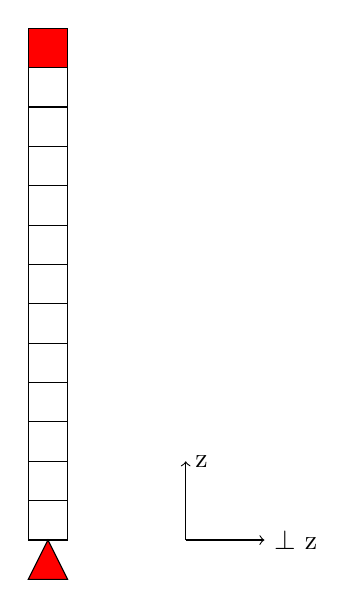
\begin{tikzpicture}
\foreach \x in {1,..., 12} \draw(0, 0.5*\x-0.5) rectangle +(.5,.5);
\filldraw[fill=red] (0, 6) rectangle +(.5,.5); 
\filldraw[fill=red] (0, -0.5) -- (0.25, 0) -- (0.5, -0.5) -- cycle;
\draw[->] (2,0) -- (2, 1) node[anchor=west] {z};
\draw[->] (2,0) -- (3, 0) node[anchor=west] {$\perp$ z};
\end{tikzpicture}
\end{center}
\caption{Geometry for test problems.}
\label{fig:exp_geometry}
\end{figure}

\subsection{Initial and Boundary Conditions}
\label{subsect:ic_bc}

The two problems, while having the same geometry, are different in their dominant physics.
One problem was designed to simulate single-phase, single-field continuous liquid flow in a standpipe; this problem will be referred to as the "Single Phase" problem.
The second problem was designed such that high-pressure liquid flashes into steam as it enters a standpipe initially filled with saturated vapor at a much lower pressure, known hereafter as the "Flashing" problem.

Table \ref{tab:ic} provides the initial conditions for the two problems.
The pressure, enthalpy, and volume-fractions for the different fields allow for a complete description of the continuity variables.
The initial velocities are set to zero.

\begin{table}[ht]
\centering
\begin{tabular}{@{}lr@{.}lr@{.}lr@{.}lr@{.}lr@{.}l@{}} \toprule
\multirow{2}{*}{Problem} & \multicolumn{2}{c}{Pressure} & \multicolumn{2}{c}{Enthalpy}             & \multicolumn{2}{c}{$\alpha_g$} & \multicolumn{2}{c}{$\alpha_l$} & \multicolumn{2}{c}{$\alpha_e$} \\ 
                         & \multicolumn{2}{c}{[psia]} & \multicolumn{2}{c}{$[\frac{\text{Btu}}{\text{lb}_{\text{m}}}]$} & \multicolumn{2}{c}{[-]}      & \multicolumn{2}{c}{[-]}      & \multicolumn{2}{c}{[-]}      \\ \midrule
Single Phase             &  200&0                       &  355&5                                   & 0&0                            & 1&0                            & 0&0 \\
Flashing                 &  200&0                       & 1198&3                                   & 1&0                            & 0&0                            & 0&0 \\ \bottomrule  
\end{tabular}
\caption{Initial conditions for test problems.}
\label{tab:ic}
\end{table}

Each of the problems has a specified pressure-enthalpy boundary condition at the top of the stand pipe and a flow-enthalpy boundary condition at the inlet of the domain.
Table \ref{tab:bc_pe} contains the pressure, enthalpy, and composition of the pressure-enthalpy reservoir. 

\begin{table}[ht]
\centering
\begin{tabular}{@{}lr@{.}lr@{.}lr@{.}lr@{.}lr@{.}l@{}} \toprule
\multirow{2}{*}{Problem} & \multicolumn{2}{c}{Pressure} & \multicolumn{2}{c}{Enthalpy}             & \multicolumn{2}{c}{$\alpha_g$} & \multicolumn{2}{c}{$\alpha_l$} & \multicolumn{2}{c}{$\alpha_e$} \\ 
                         & \multicolumn{2}{c}{[psia]} & \multicolumn{2}{c}{$[\frac{\text{Btu}}{\text{lb}_{\text{m}}}]$} & \multicolumn{2}{c}{[-]}      & \multicolumn{2}{c}{[-]}      & \multicolumn{2}{c}{[-]}      \\ \midrule
Single Phase             &  200&0                       &  355&5                                   & 0&0                            & 1&0                            & 0&0 \\
Flashing                 &  200&0                       & 1198&3                                   & 1&0                            & 0&0                            & 0&0 \\ \bottomrule  
\end{tabular}
\caption{Outlet pressure-enthalpy boundary conditions for test problems.}
\label{tab:bc_pe}
\end{table}

The flow-enthalpy boundary condition describes the thermodynamic state of the inflowing fluid and its flow rate.
Table \ref{tab:bc_fe} describes the inlet boundary condition for the two problems.

\begin{table}[ht]
\centering
\begin{tabular}{@{}lr@{.}lr@{.}lr@{.}lr@{.}lr@{.}l@{}} \toprule
\multirow{2}{*}{Problem} & \multicolumn{2}{c}{Pressure} & \multicolumn{2}{c}{Enthalpy}             & \multicolumn{2}{c}{$\alpha_g$} & \multicolumn{2}{c}{$\alpha_l$} & \multicolumn{2}{c}{$\alpha_e$} \\ 
                         & \multicolumn{2}{c}{[psia]} & \multicolumn{2}{c}{$[\frac{\text{Btu}}{\text{lb}_{\text{m}}}]$} & \multicolumn{2}{c}{[-]}      & \multicolumn{2}{c}{[-]}      & \multicolumn{2}{c}{[-]}      \\ \midrule
Single Phase             &  200&0                       &  355&5                                   & 0&0                            & 1&0                            & 0&0 \\
Flashing                 & 1000&0                       &  542&6                                   & 1&0                            & 0&0                            & 0&0 \\ \bottomrule  
\end{tabular}
\caption{Inlet f	low-enthalpy boundary conditions for test problems.}
\label{tab:bc_fe}
\end{table}

The specified mass flow, $\dot{m}(t)$, at the bottom of the channels is the same for both problems. 
The is a time-dependent function give by \eqref{eqn:bc_time_func_single}.

\begin{equation}
\label{eqn:bc_time_func_single}
\dot{m}(t) = \left\{
\begin{array}{cclrcll}
 0.0           & [\frac{\text{lb}_{\text{m}}}{\text{s}}] & , &         & t & \leq 1 &[\text{s}] \\
 0.5 ( t - 1)  & [\frac{\text{lb}_{\text{m}}}{\text{s}}] & , & 1 [\text{s}] < & t & \leq 2 &[\text{s}] \\
 0.5           & [\frac{\text{lb}_{\text{m}}}{\text{s}}] & , &         & t & > 2    &[\text{s}]
\end{array}\right.
\end{equation}

Both problems adjust their initial pressure distribution to account for hydrostatic head, which is not specified in the input files.
The \cobra{} input files for both problems can be found in \app{app:input_decks}.

\subsection{Results}
\label{subsect:results}

The two problems were set up so that the maximum allowable time-step was varied.
Each problem was run with the following maximum allowable time-steps: 1 [s], 0.1 [s], 0.01 [s], 0.001 [s], 0.0001 [s], and 0.00001 [s]. 
For the legacy runs, the scaled residuals were evaluated after a single Newton-step.
For the nonlinear runs, the scaled nonlinear residuals were evaluated at the end of the Newton-loop.
The nonlinear convergence criteria used for the nonlinear runs are described in \sect{sect:nl_cobra}.
The temporal convergence metric was evaluated during post-processing.

In total, there were twenty-four simulations run.
The two different problems were each run at six different maximum time-step sizes on each of the two version of \cobra.
Of the twenty-four simulations run, the legacy mode simulation of flashing at a time-step size of 1 [s] failed to run to completion.

\comment{Does the temporal convergence metric provide a quantifiable measure for a converged time-step size insensitive solution?}

The convergence metric will be used to determine if a qualitative temporal-convergence determination can lead to the acceptance of solution that is not nonlinearly converged.
For each of the test cases, these variables were compared at different time-steps.
First, the 1 [s] max time-step legacy simulation of the flashing problem failed to run.
The time-step limiting procedure outlined \sect{sect:algorithmic_concerns} was unable to prevent too large of changes to the independent parameters by reducing the time-step.
This caused the problem to try to run below a the minimum allowable time-step size, which resulted in the software aborting.
However, the nonlinearly convergent \cobra{} was able to run at a 1 [s] time-step.
Both versions of \cobra{} are subject to the same limits on change of independent variables.

\fig{fig:flashing_1em1} shows the gaseous volume fraction 2 [in] from the inlet of the stand pipe as a function of time for a max \dt{} of 1.0E-1 [s] for both the legacy and the nonlinear solvers.

\begin{figure}[h!t]
\centering
\subfloat[Solution at $\Delta t_{\text{MAX}} = $1.0E-1 {[s]}]{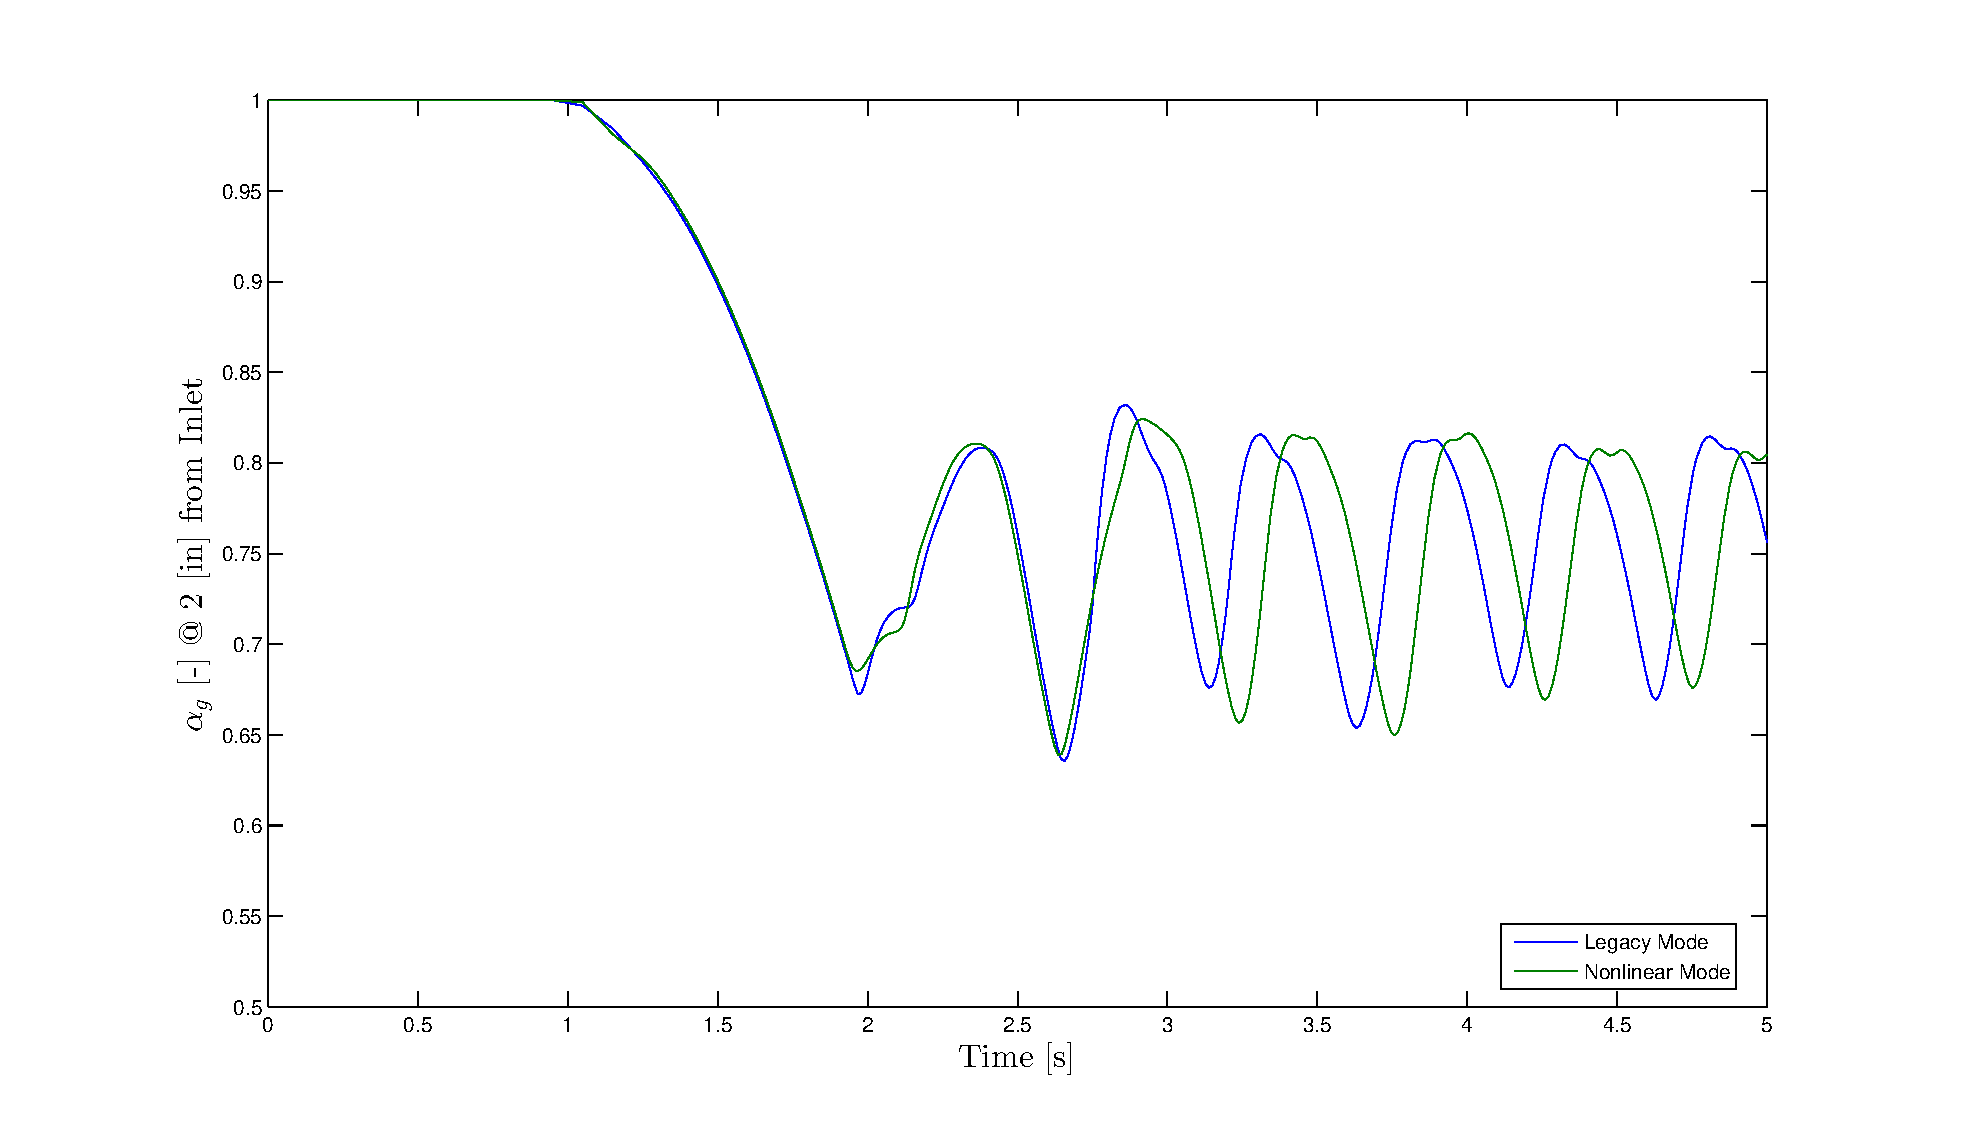
\includegraphics[width=0.49\textwidth]{images/flashing_1em1.eps}
\label{fig:flashing_1em1}}
\subfloat[Solution at $\Delta t_{\text{MAX}} = $1.0E-5 {[s]}]{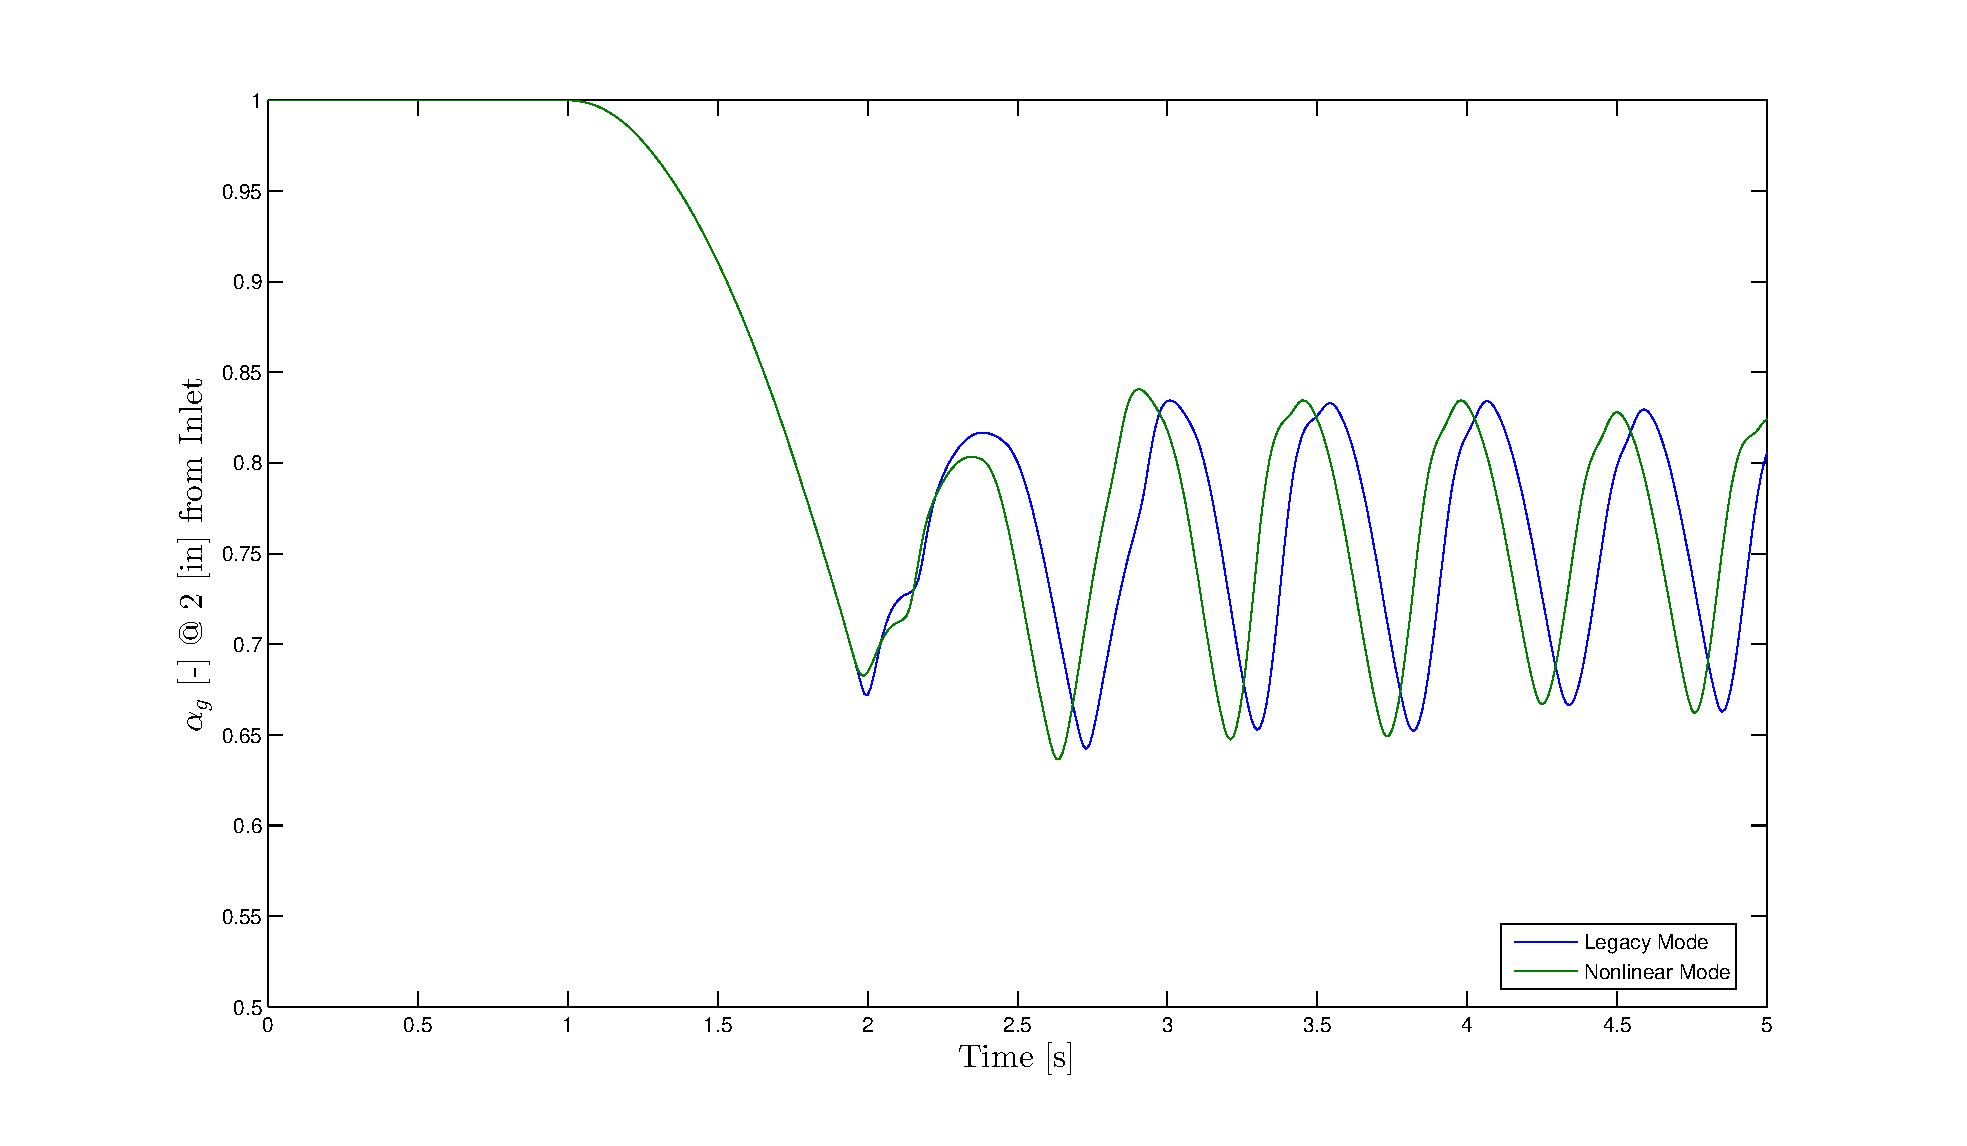
\includegraphics[width=0.49\textwidth]{images/flashing_1em5.eps}
\label{fig:flashing_1em5}}
\caption[Flashing solution at $\Delta t_{\text{MAX}}$ = 1.0E-1 {[s]}and 1.0E-5 {[s]}]{Flashing solution at $\Delta t_{\text{MAX}}$ = 1.0E-1 {[s]} and 1.0E-5 {[s]}.}
\label{fig:flashing_compare_1}
\end{figure}

Note that the nonlinearly resolved solution is qualitatively different than the traditional single-shot solution, \fig{fig:flashing_1em1}.
Even as the time-step size is reduced, this discrepancy does does disappear, \fig{fig:flashing_1em5}.

The two solutions do not converge to the same solution as the time-step size was reduced.
Notice however, that the solution to the flashing problem produced by the nonlinear mode of \cobra{}, \fig{fig:nl_mode_flashing}, varies less as the time-step size is reduced that that produced by the legacy mode, \fig{fig:cobra_mode_flashing}.
However, both \fig{fig:cobra_mode_flashing} and \fig{fig:nl_mode_flashing} show that as the time-step size is reduced the solution becomes more time-step size insensitive.

\begin{figure}[h!t]
\centering
\subfloat[Legacy mode solution.]{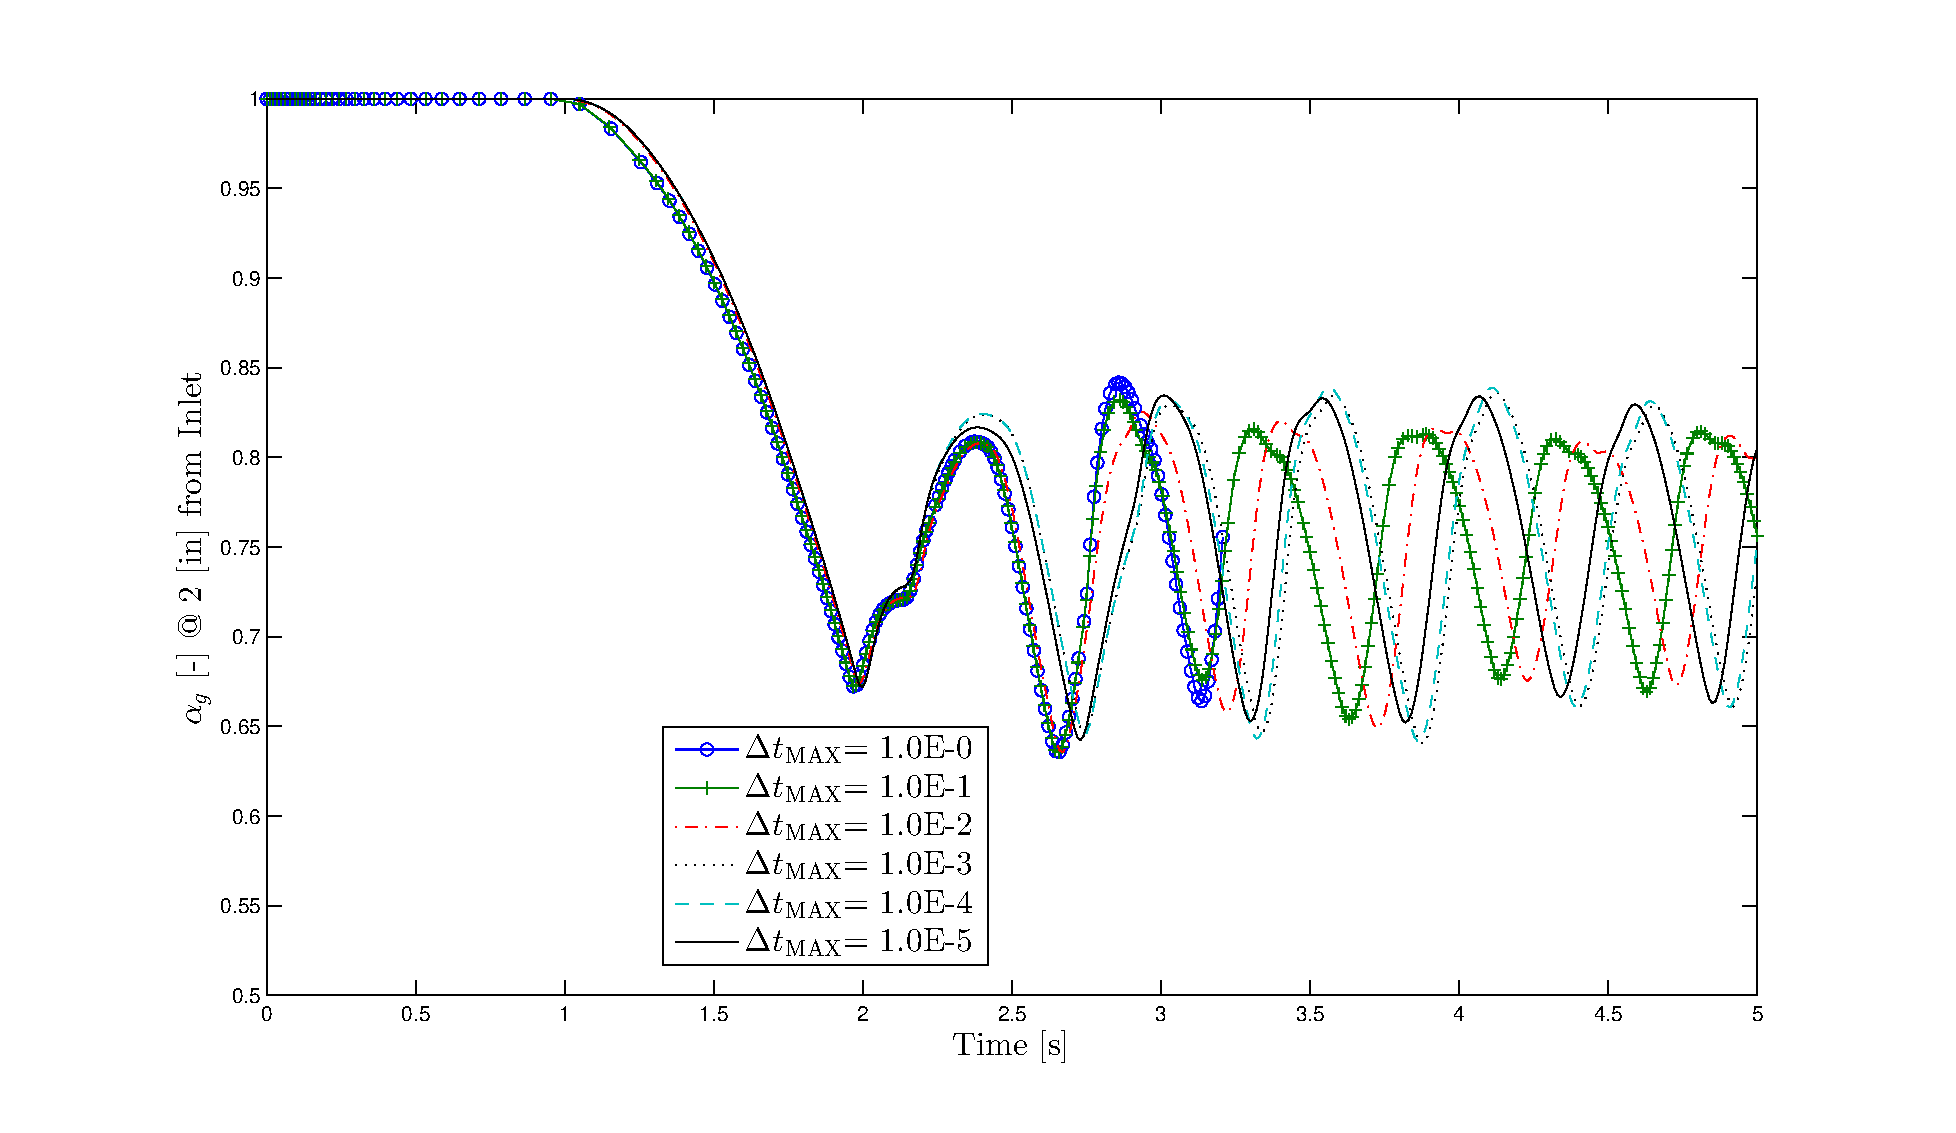
\includegraphics[width=0.49\textwidth]{images/cobra_flashing_al_2in.eps}
\label{fig:cobra_mode_flashing}}
\subfloat[Nonlinear mode solution.]{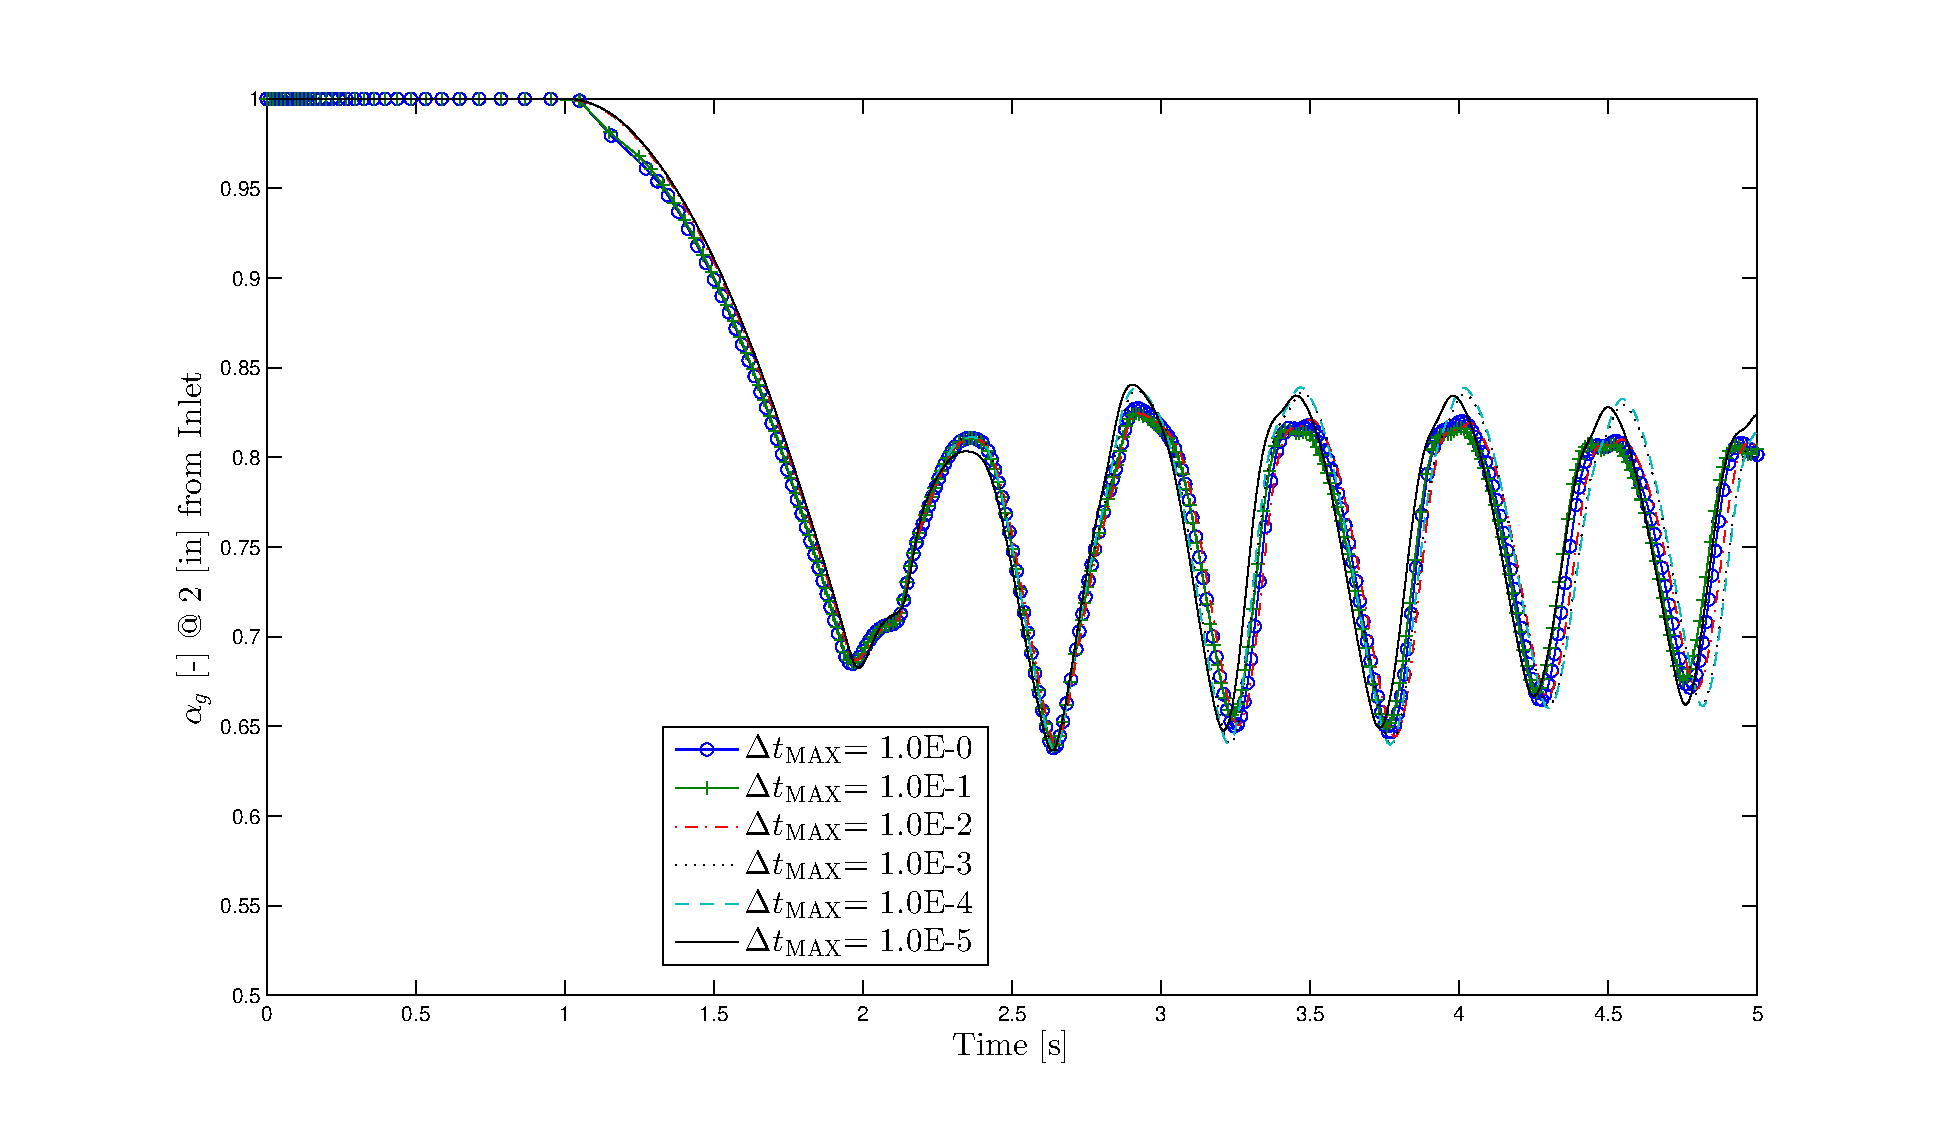
\includegraphics[width=0.49\textwidth]{images/nl_flashing_al_2in.eps}
\label{fig:nl_mode_flashing}}
\caption{Flashing simulation.}
\label{fig:flashing_solutions_1}
\end{figure}

The two modes of \cobra{}, when applied to the same problem that contains highly nonlinear physics, produce two different time-step size invariant solutions.
These two solutions reach time-step size invariance at different time-step sizes.
The solution produced by the nonlinear mode at 1 [s] $\Delta t_{\text{MAX}}$ is qualitatively as close to that produced with a 0.1 [s] $\Delta t_{\text{MAX}}$, \fig{fig:nl_flashing_compare}, as the legacy mode simulations at 1.0E-3 [s] and 1.0E-4 [s] $\Delta t_{\text{MAX}}$ are to each other, \fig{fig:cobra_flashing_compare}.

\begin{figure}[h!t]
\centering
\subfloat[Nonlinear mode solution.]{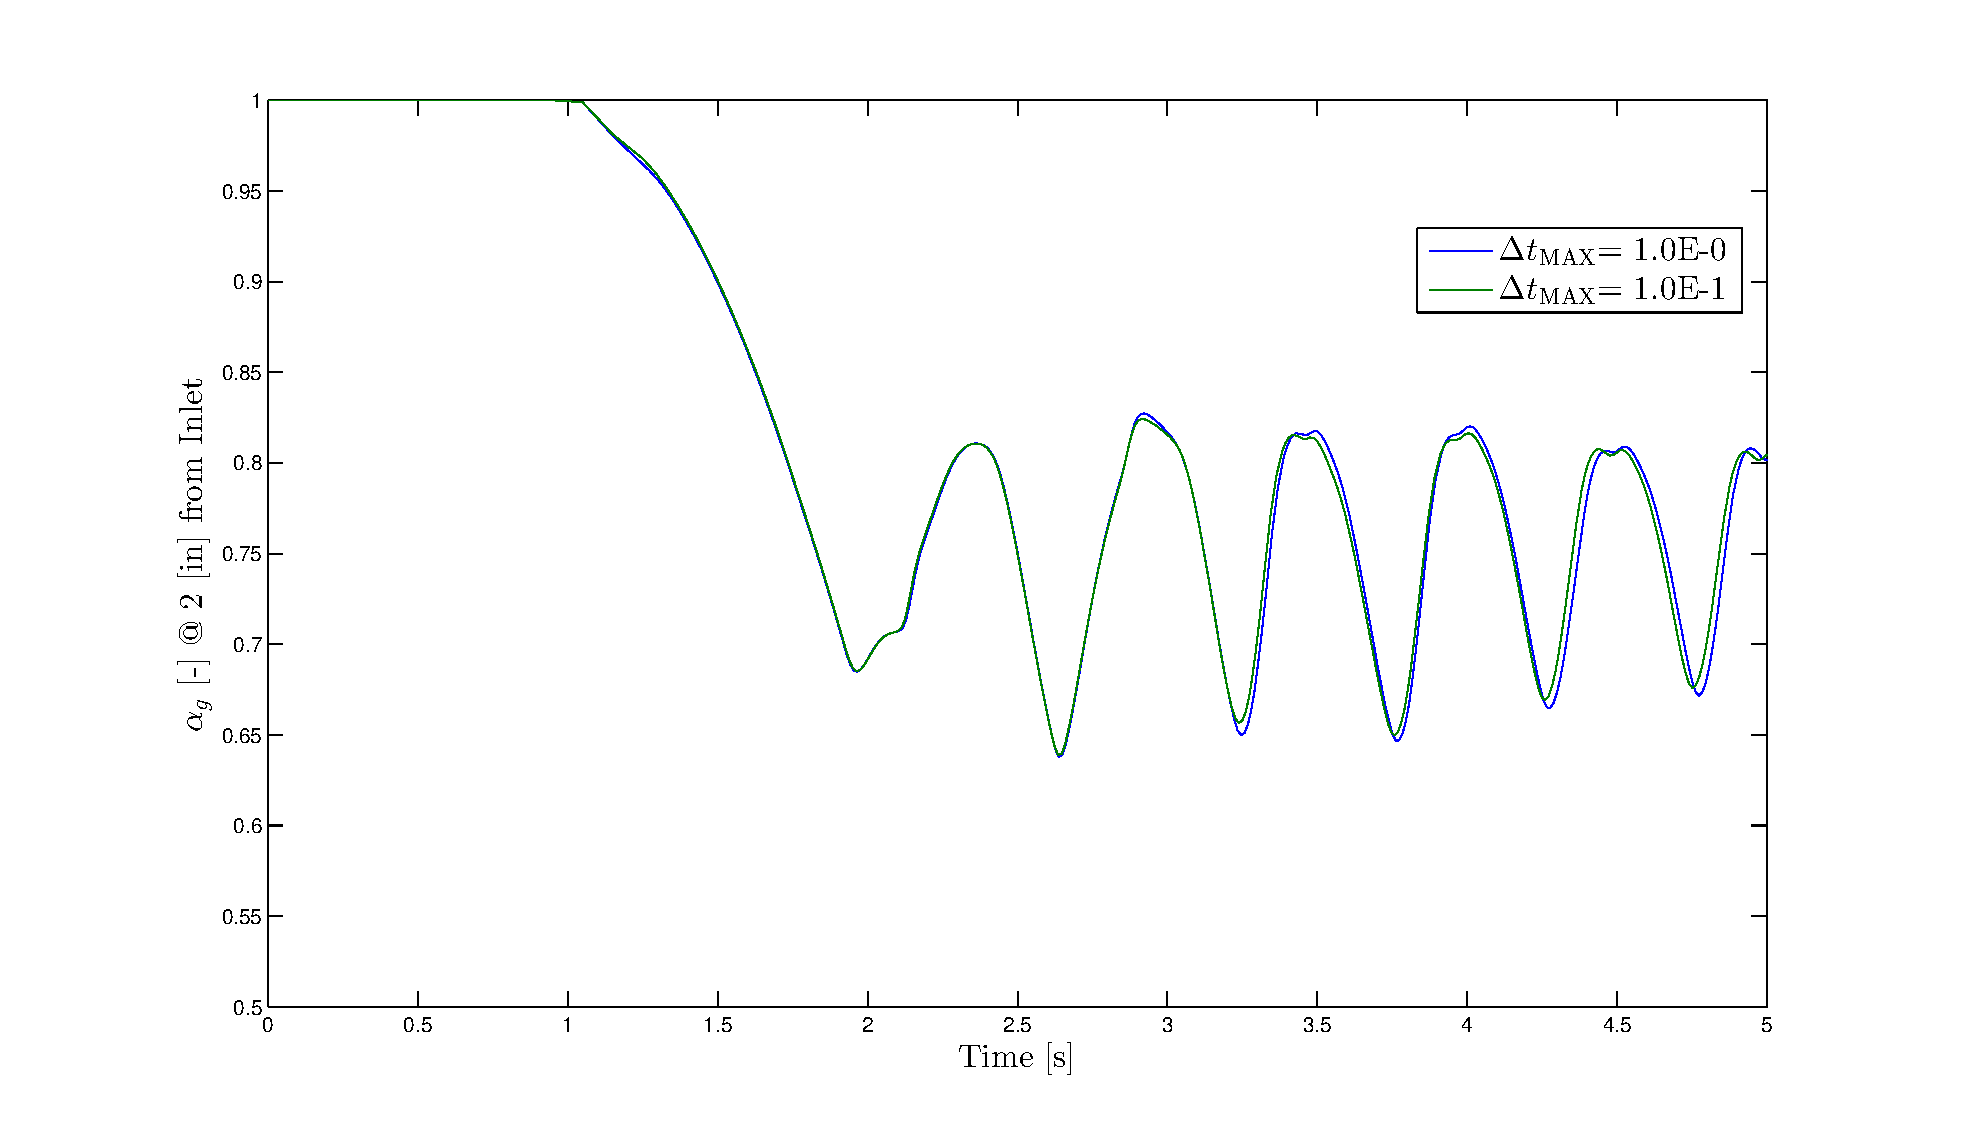
\includegraphics[width=0.49\textwidth]{images/nl_flashing_1em0_1em1.eps}
\label{fig:nl_flashing_compare}}
\subfloat[Legacy mode solution.]{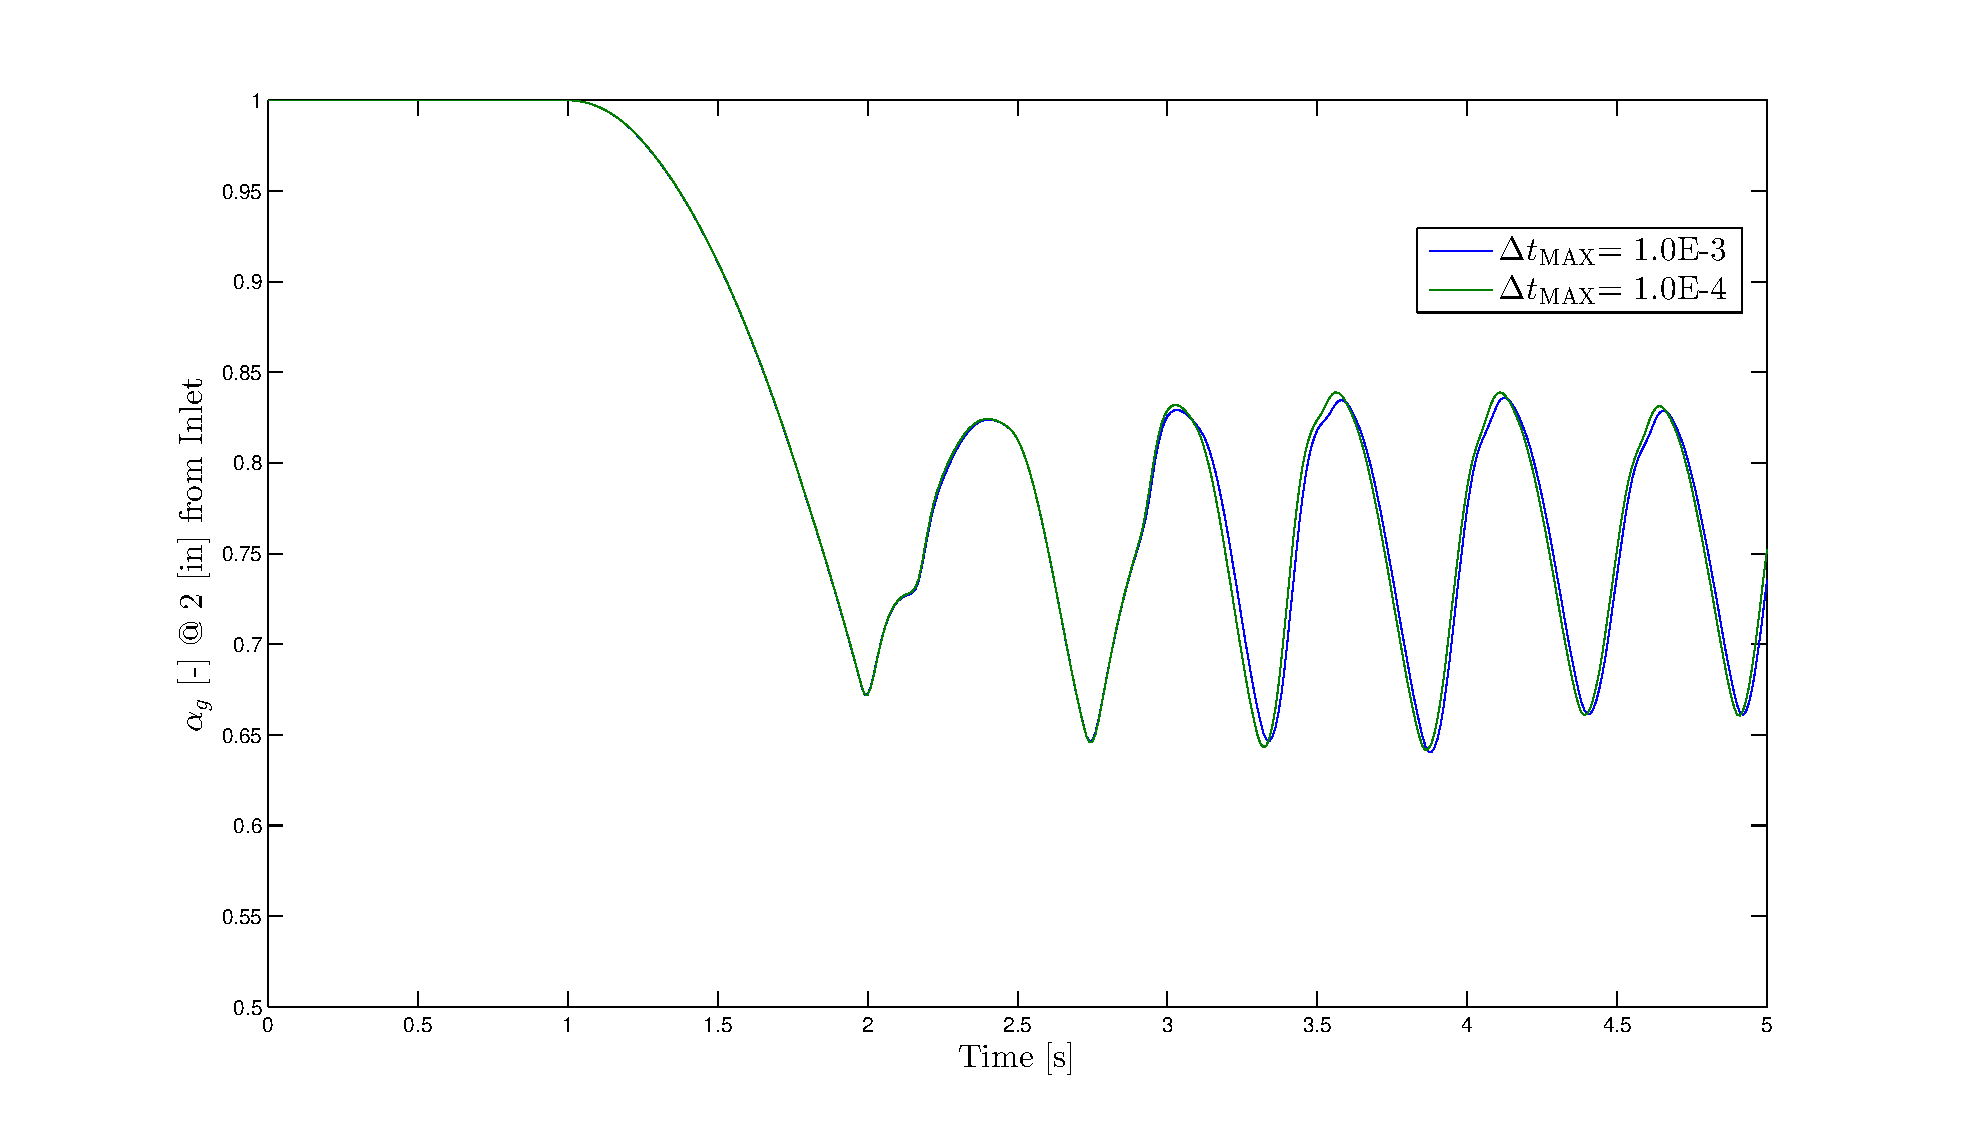
\includegraphics[width=0.49\textwidth]{images/cobra_flashing_1em3_1em4.eps}
\label{fig:cobra_flashing_compare}}
\caption{Time-step size insensitive Flashing solutions.}
\label{fig:flashing_res_comp_1}
\end{figure}

The time-step size insensitive solution produced by the nonlinearly convergent solver in \cobra{} occurs at maximum time-step size three orders of magnitude greater than that achieved by the single-shot linearization solver in \cobra{}.
An examination of the nonlinear residual over the course of the transient provides insight into why this behavior is observed.
The scaled nonlinear residual for the legacy Flashing problem indicates that even for small time-step sizes, the solution obtained still does not satisfy the discrete nonlinear equations, \fig{fig:legacy_flashing_residual}.
This is in contrast to the nonlinear flashing problem, which shows a lower nonlinear residual over the course of the simulation, \fig{fig:nonlinear_flashing_residual}.

\begin{figure}[h!t]
\centering
\subfloat[Nonlinear mode residuals.]{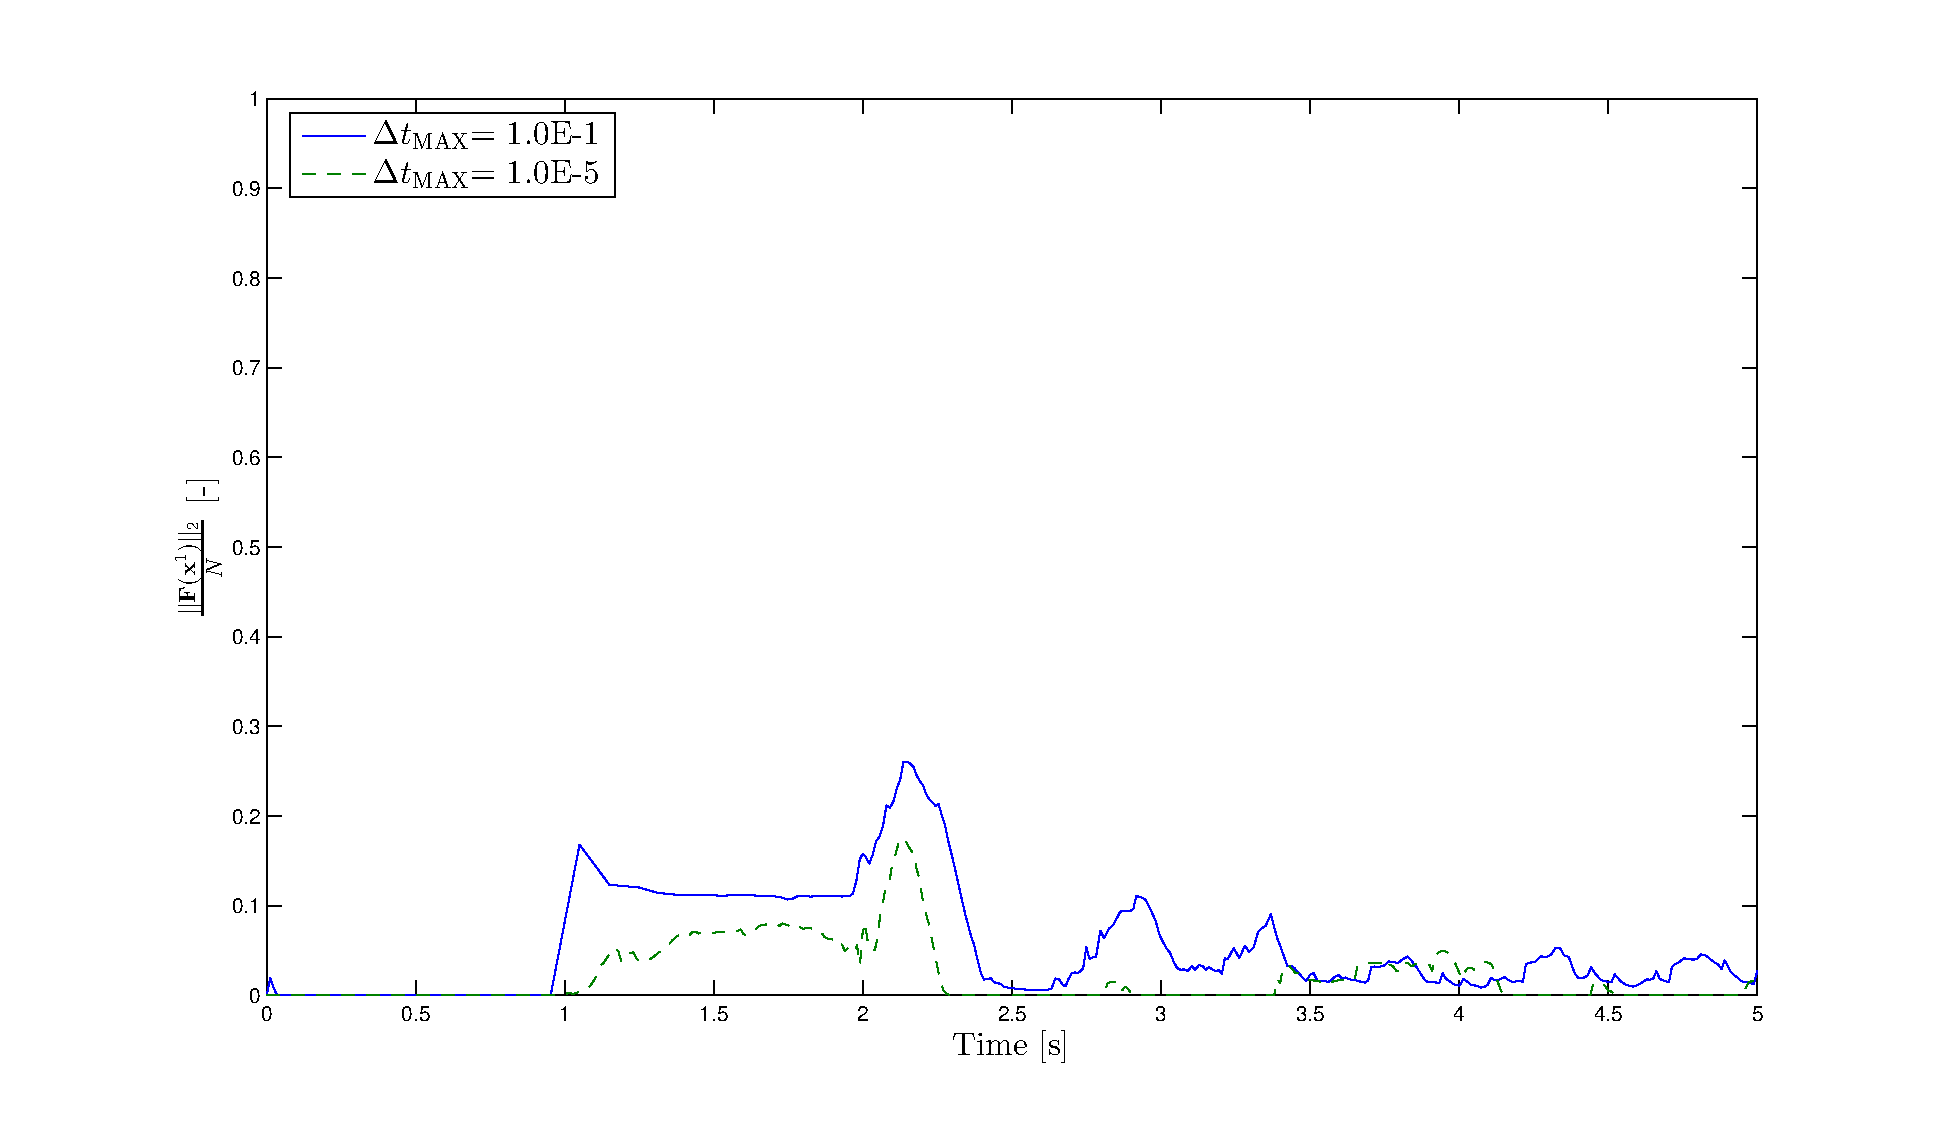
\includegraphics[width=0.49\textwidth]{images/cobra_flashing_res_compare.eps}
\label{fig:legacy_flashing_residual}}
\subfloat[Legacy mode residuals.]{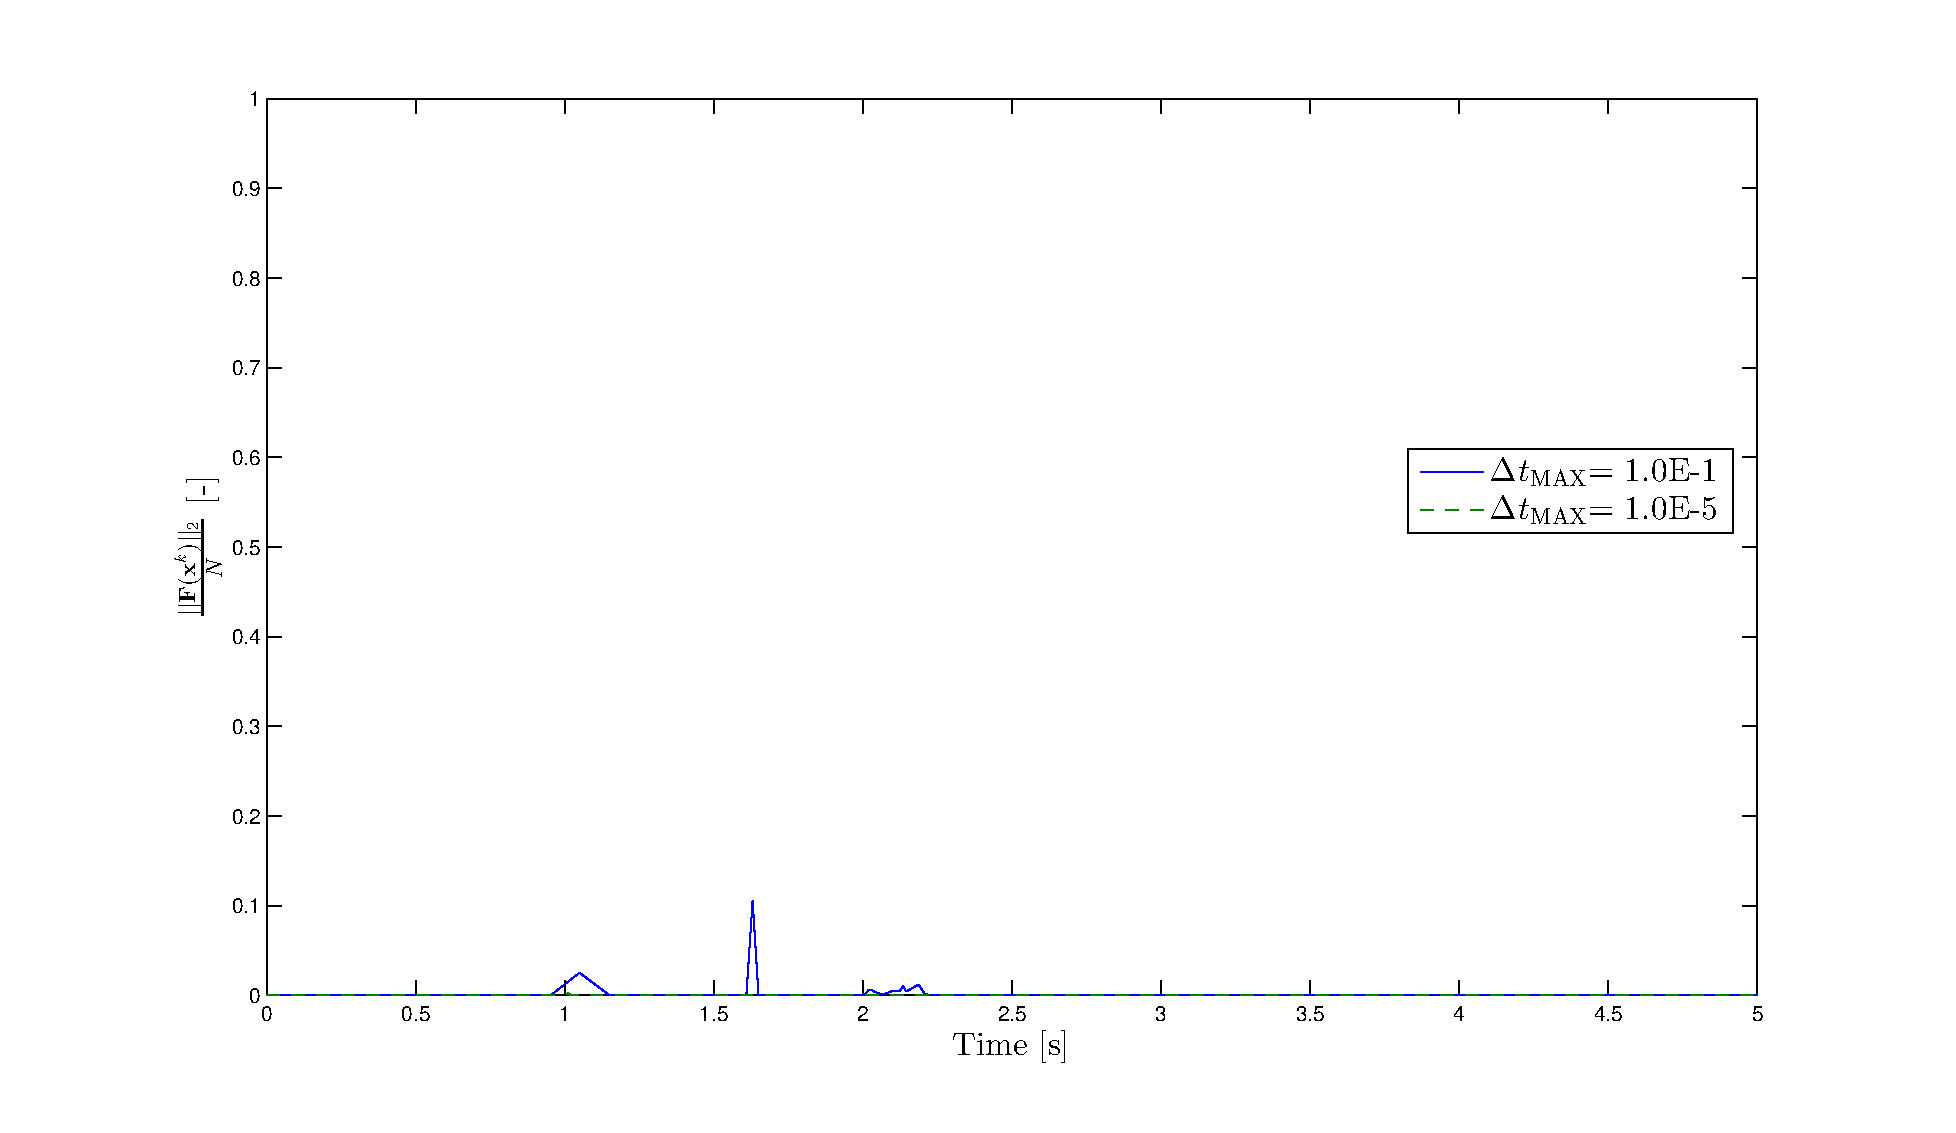
\includegraphics[width=0.49\textwidth]{images/nl_flashing_res_compare.eps}
\label{fig:nonlinear_flashing_residual}}
\caption[Flashing residual at $\Delta t_{\text{MAX}}$ = 1.0E-1 {[s]}and 1.0E-5 {[s]}]{Flashing residual at $\Delta t_{\text{MAX}}$ = 1.0E-1 {[s]} and 1.0E-5 {[s]}.}
\label{fig:flashing_compare_2}
\end{figure}

The reduction in the residual exhibited by the legacy mode solution, \fig{fig:legacy_flashing_residual}, shows that the reduction of the time-step size now reduces two errors.
As the time-step size is reduced, the nonlinear physics are being better resolved; however, even for small time-step sizes, the nonlinear residual is still large compared to the nonlinear residual of the nonlinearly convergent simulation, \fig{fig:nonlinear_flashing_residual}.
The residuals of the nonlinearly convergent \cobra{} mode are non-zero at certain portions of the simulation at large time-step sizes.
There are several possibilities as to why the residuals are non-zero.
The convergence criteria outlined in \sect{sect:nl_cobra} include two paths through which Newton's method may terminate while not having a zero residual.
The first is that the $k_{\text{MAX}}$ may be too small, terminating the iterative process prior to a solution being obtained.
The second is that the norm of the scaled independent parameter update vector may be below the convergence threshold.
A concern is that the update vector is the vector based upon the limiting of the independent parameters.
So, it may be impossible for the algorithm to reach a nonlinearly converged solution without pushing a parameter outside of the acceptable limits.
This behavior needs additional investigation to determine both the cause and the impact upon the algorithmic frame work.

To examine efficacy of the the temporal convergence criteria, both the average and moment based temporal convergence criteria were evaluated for each of the twenty-three successful simulations.

One way to quantify the difference between the solutions is by measuring the nonlinear residual metric outlined in \ref{sect:temporal_convergence}.
This metric provides a measure of how poorly the discrete nonlinear equations are being solved at every time-step in the transient.
The resolution of the nonlinear residual allows for a solution that is less sensitive to time-step size selection than the solution that does not resolve the nonlinear residual.

See \tab{tab:flashing_criteria} and \tab{tab:single_criteria} for the data.

\begin{table}[h!t]
\centering
\begin{tabular}{@{}l r@{.}l r@{.}l r@{.}l r@{.}l @{}}
\toprule
& \multicolumn{4}{c}{$\tilde{R}$} & \multicolumn{4}{c}{$\tilde{R}_{\text{M}}$}  \\
$\Delta t_{\text{MAX}}$ & \multicolumn{2}{c}{Legacy} & \multicolumn{2}{c}{Nonlinear} & \multicolumn{2}{c}{Legacy}& \multicolumn{2}{c}{Nonlinear}  \\
\midrule
1.0    & \multicolumn{2}{c}{-} & 1&177E-3 & \multicolumn{2}{c}{-} & 6&885E-4 \\
1.0E-1 & 5&487E-2 & 1&141E-3 & 5&044E-2 & 6&730E-4 \\
1.0E-2 & 4&960E-2 & 3&413E-4 & 4&570E-2 & 2&511E-4 \\
1.0E-3 & 3&172E-2 & 2&669E-4 & 2&372E-2 & 1&975E-4 \\
1.0E-4 & 2&504E-2 & 1&346E-4 & 1&838E-2 & 8&974E-5 \\
1.0E-5 & 2&166E-2 & 5&075E-5 & 1&922E-2 & 4&581E-5 \\
\bottomrule  
\end{tabular}
\caption{Nonlinear convergence metrics for Flashing problem.}
\label{tab:flashing_criteria}
\end{table}

The average metric for the legacy flashing problem shows that the single-shot case has unresolved nonlinearities of greater magnitude than the nonlinear case.
This is expected.
Other scientist have noted this behavior.

The single-phase problem should be relatively linear.
As such, the solution produced by the linear solver should be the same as that produced by the linear solver.
In addition, the solution should be time-step size insensitive from the beginning.

It should also show that the solution for both the single-shot and the nonlinear versions of \cobra{} produced the same result.
The nonlinear \cobra{} did not produce the same results.
This is where I show the blowup picture of the oscillatory solution.
I also show how the residual increases as the time-step size is decreased.
It produced solutions with bounded oscillations at smaller time-step sizes.
In addition the residuals appear to be growing with smaller time-steps.
I do not know why at the moment.
This poor behavior could be the result of multiple issues.
One possibility is the inconsistency between the scaled update vector used in the line-search algorithm and  the one used in the Newton loop convergence criteria.
Another possibility is the limiters used in the operator-based scaling were chosen poorly.

\begin{table}[h!t]
\centering
\begin{tabular}{@{}l r@{.}l r@{.}l r@{.}l r@{.}l @{}}
\toprule
& \multicolumn{4}{c}{$\tilde{R}$} & \multicolumn{4}{c}{$\tilde{R}_{\text{M}}$}  \\
$\Delta t_{\text{MAX}}$ & \multicolumn{2}{c}{Legacy} & \multicolumn{2}{c}{Nonlinear} & \multicolumn{2}{c}{Legacy}& \multicolumn{2}{c}{Nonlinear}  \\
\midrule
1.0    & 3&149E-3 & 1&700E-3 & 1&485E-3 & 1&070E-4 \\
1.0E-1 & 2&866E-3 & 1&700E-3 & 1&287E-3 & 1&070E-4 \\
1.0E-2 & 3&412E-4 & 1&357E-3 & 1&417E-4 & 7&701E-5 \\
1.0E-3 & 2&207E-4 & 4&584E-4 & 8&805E-5 & 1&178E-4 \\
1.0E-4 & 1&672E-4 & 1&588E-3 & 1&834E-5 & 4&958E-5 \\
1.0E-5 & 5&493E-4 & 2&758E-4 & 1&916E-5 & 8&939E-5 \\
\bottomrule  
\end{tabular}
\caption{Nonlinear convergence metrics for Single Phase problem.}
\label{tab:single_criteria}
\end{table}

\section{Review}
\label{sect:review}

In review, the single-shot semi-implicit \cobra{} software was converted to a nonlinearly convergent, semi-implicit algorithm.
An operator-based scaling was introduced and implemented into the nonlinear \cobra{}.
Deficiencies were identified with the current implementation of the operator-based scaling.
A metric to quantify the nonlinear convergence of a temporally converged simulation was developed and implemented.
Tests indicated that a time-step size insensitive solution may not be nonlinearly converged and can be an incorrect solution to the nonlinear discrete equations.